\chapter{Interaction potentials and thermostats}

\section{Canonical fluctuations}

The exercise asked to show that the temperature fluctuations in the canonical
ensemble are
\begin{equation}
  \frac{\sigma_{T_{K}}^{2}}{\expval{T_{K}}^{2}} = \frac{\expval{T_{K}^{2}} -
  \expval{T_{K}}^{2}}{\expval{T_{K}}^{2}} = \frac{2}{3N},
\end{equation}
where the kinetic temperature $T_{K}$ is given by
\begin{equation}
  T_{K} = \frac{1}{3N k_{\mathrm{B}}} \sum_{i=1}^{N} m_{i} v_{i}^{2}.
\end{equation}

First, denoting the kinetic energy with $E_{K}$, we can rewrite $T_{K}$ as
\begin{equation}
  T_{K} = \frac{2E_{K}}{3N k_{\mathrm{B}}}, \quad \text{with }
  E_{K} = \frac{1}{2} \sum_{i=1}^{N} m_{i} v_{i}^{2}.
  \label{eq:tk-ek}
\end{equation}
At this point we need the variance of $E_{K}$: we can start from the
equipartition theorem
\begin{equation}
  \expval{E_{K}} = \frac{3N}{2 \beta},
\end{equation}
and being in the canonical ensemble we can derive with respect to $\beta$:
\begin{equation}
  \sigma_{E_{K}}^{2} = \expval{E_{K}^{2}} - \expval{E_{K}}^{2} =
  -\pdiff{}{\beta} \expval{E_{K}} = -\frac{3N}{2} \pdiff{}{\beta}\frac{1}{\beta}
  = \frac{3N}{2 \beta^{2}}.
\end{equation}
Putting this into \cref{eq:tk-ek} we get
\begin{equation}
  \sigma_{T_{K}}^{2} = \expval{T_{K}^{2}} - \expval{T_{K}}^{2} =
  \frac{4}{9N^{2} k_{\mathrm{B}}^{2}} \frac{3N}{2 \beta^{2}} = \frac{2}{3N
  k_{\mathrm{B}}^{2} \beta^{2}}.
\end{equation}
By squaring \cref{eq:tk-ek} we also get $\expval{T_{K}}^{2}$, so, finally:
\begin{equation}
  \frac{\sigma_{T_{K}}^{2}}{\expval{T_{K}}^{2}} = \frac{2}{3N k_{\mathrm{B}}^{2}
  \beta^{2}} \frac{9 N^{2} k_{\mathrm{B}}^{2}}{4 \expval{E_{K}}^{2}} =
  \frac{3N}{2 \beta^{2}} \frac{4 \beta^{2}}{9 N^{2}} = \frac{2}{3N}.
\end{equation}

\section{Lennard-Jones fluid in the microcanonical ensemble}

\begin{sourcefiles}
  \item[Source codes] src/102\_lennard\_jones.c, src/moldyn/integration.c,
    src/moldyn/integration.h, src/moldyn/observables.c,
    src/moldyn/observables.h, src/moldyn/parameters.c, src/moldyn/parameters.h
  \item[Analysis script] src/102\_lennard\_jones.R
  \item[Executable] exe/102\_lennard\_jones
\end{sourcefiles}

The six source files inside the \texttt{src/moldyn} directory follow a similar
structure to those discussed in \cref{ch:offlat}. \texttt{parameters.c} and
\texttt{parameters.h} function similarly to their previously mentioned
counterparts, though they now include a larger set of parameters. The parameters
listed in \cref{ex:082} are still present, with the exception that
\texttt{max\_disp} now refers only to the (optional) Monte Carlo equilibration
phase. The additional parameters are:
\begin{description}[font=\normalfont\ttfamily]
  \item[r\_cut] cutoff radius for the potential.
  \item[step\_size] for the Molecular Dynamics simulation.
  \item[eq\_type] specifies either \texttt{mc} (Monte Carlo) or \texttt{md}
    (Molecular Dynamics) as the equilibration method.
  \item[num\_eq\_steps] number of Monte Carlo sweeps or \abbr{md} steps in the
    equilibration phase. The total number of steps in the simulation is
    therefore $\text{\texttt{num\_eq\_steps}} + \text{\texttt{num\_steps}}$.
  \item[thinning] if larger than \num{1}, the program writes to file every
    \texttt{thinning} non-equilibration steps.
  \item[rdf\_max\_radius] maximum inter-particle distance considered in the
    calculation of the radial distribution function.
  \item[rdf\_num\_bins] number of bins used for the radial distribution
    function.
\end{description}

As for \cref{ex:082}, the function \texttt{initialize()}, defined in
\texttt{integration.c}, is responsible for initializing the particles’ positions
either in a random configuration or a (cubic) lattice
structure. Additionally, it generates initial velocities from a Maxwell--Boltzmann
distribution at the chosen temperature, enforcing the total momentum to zero.

Following this, the \texttt{equilibrate()} function may be invoked, performing
\texttt{num\_eq\_steps} equilibration steps as specified by the
\texttt{eq\_type} parameter. This function requires pointers to a
\texttt{compute\_energy\_delta()} function for the Monte Carlo procedure, and
\texttt{compute\_forces()} for the Molecular Dynamics. The latter is also passed
to the subsequent function, \texttt{step()}, which carries out a single
integration step of the Velocity Verlet algorithm.\footnote{The \texttt{step()}
function also calls the \texttt{static} function \texttt{thermostat()}, which
will be covered in the next section. If the parameter \texttt{thermostat} is
unset -- or set to \enquote{none} -- the function does nothing.} The
Lennard-Jones implementations of the \texttt{compute} functions are located in
main file \texttt{102\_lennard\_jones.c}.

Lastly, the \texttt{update\_obs()} function, defined in \texttt{observables.c},
updates the values for kinetic energy, potential energy, kinetic temperature,
and the \texttt{rdf\_num\_bins} samples of the radial distribution function.
These quantities are stored in a \texttt{struct observables}, which is defined
in \texttt{observables.h}.

With this setup, I ran a set of simulations varying the cutoff radius and
keeping fixed $L = \num{10}$, $\rho = \num{0.2}$ and $T = \num{1}$ (all in
Lennard-Jones reduced units). Each simulation lasted \num{10000} Verlet steps --
after \num{1000} Monte Carlo sweeps for equilibration -- with a thinning of
\num{10} and repeated for \num{10} realizations. I varied $r_{\mathrm{cut}}$
from $2^{1/6}$ to \num{3.9} with steps of \num{0.2}, in units of $\sigma$.

\Cref{fig:102a} shows the resulting potential energy distributions overlaid for
comparison. In general, the distribution broadens and the average decreases as
the cutoff radius increases. This behaviour is expected, as longer-distance
interactions lead to a more tightly bound system. In contrast, at smaller values
of $r_{\mathrm{cut}}$, the fluid behaves almost like a non-interacting gas. This
trend is further supported by the evolution of the radial distribution function,
shown in \cref{fig:102b,fig:102c}. When $r_{\mathrm{cut}}$ is small, $g(r)$
displays a single peak around the equilibrium distance $2^{1/6}$, followed by a
rapid decay to \num{1}. However, with larger cutoff radii, the first peak grows,
and a second one appears, indicating a transition to a more liquid phase.

\begin{figure}
  \centering
  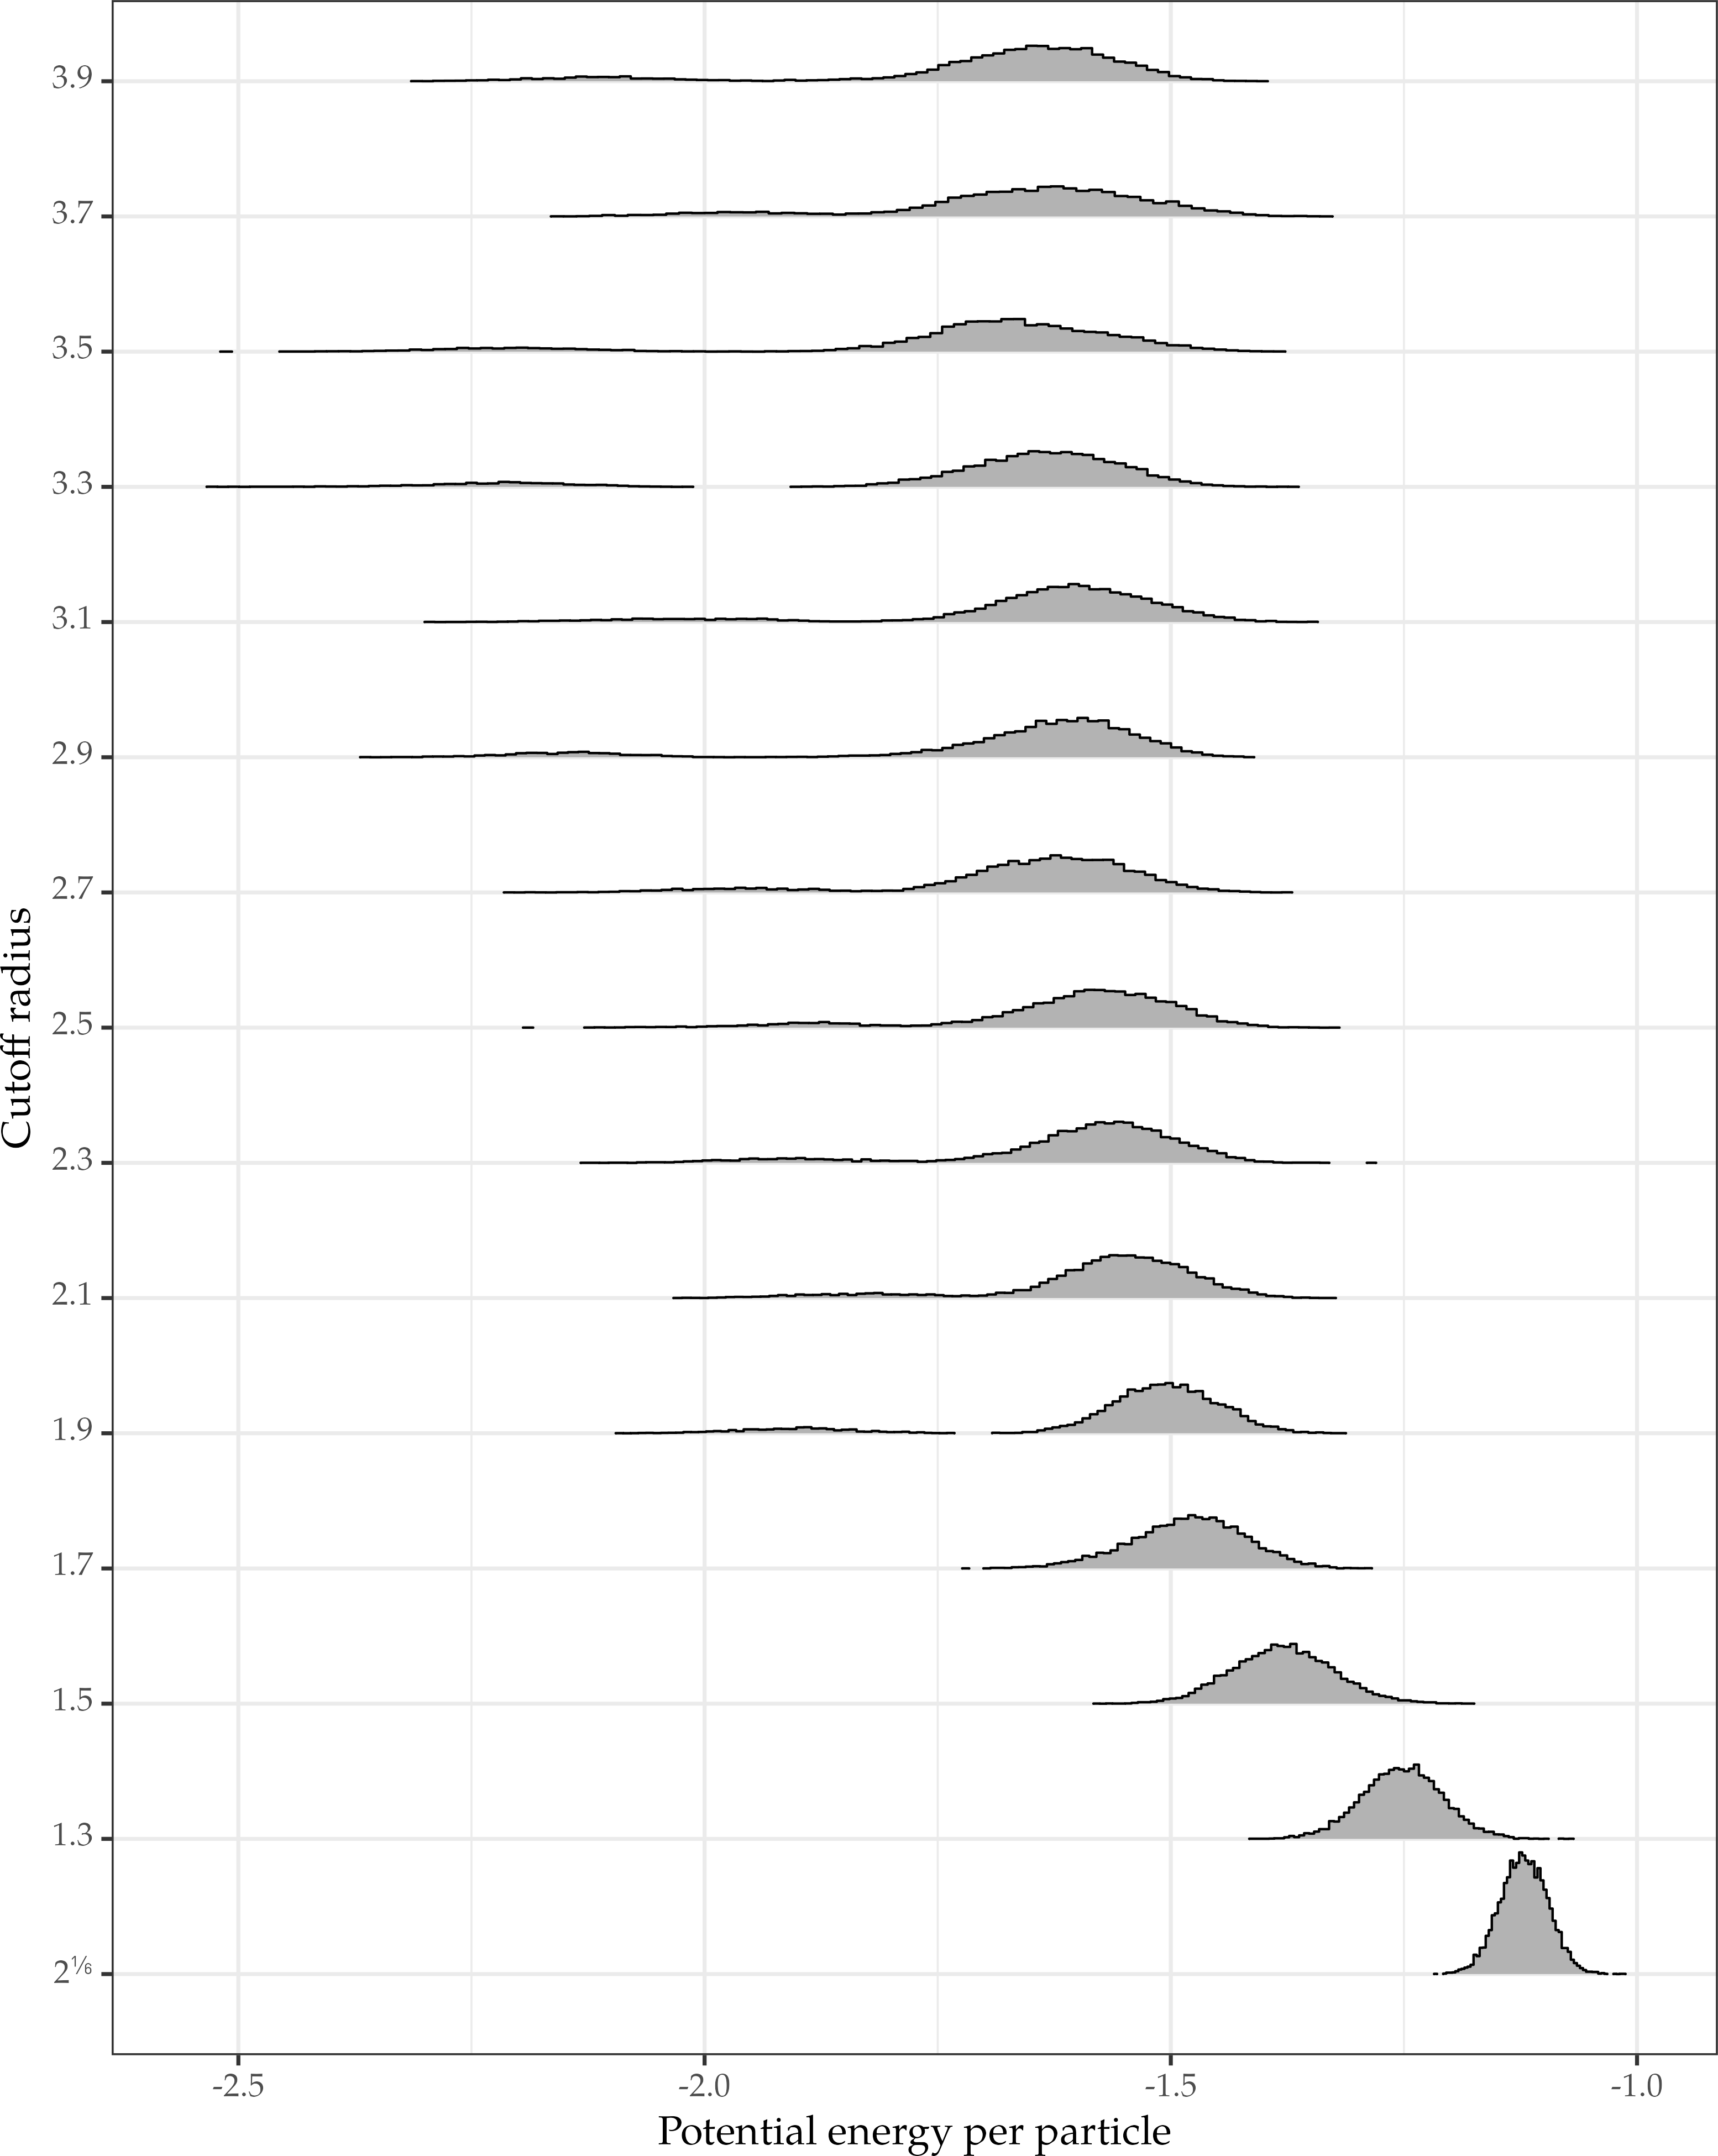
\includegraphics{img/102a}
  \caption{potential energy distributions at different cutoff radii for a
    Lennard-Jones system of \num{200} particles, box size $L = \num{10}$ and
    temperature $T = \num{1}$. Each histogram is the aggregate of \num{10}
    realizations with \num{10000} \abbr{md} steps sampled every \num{10}, after
    an equilibration phase of \num{1000} \abbr{mc} sweeps.}
  \label{fig:102a}
\end{figure}

\begin{figure}
  \centering
  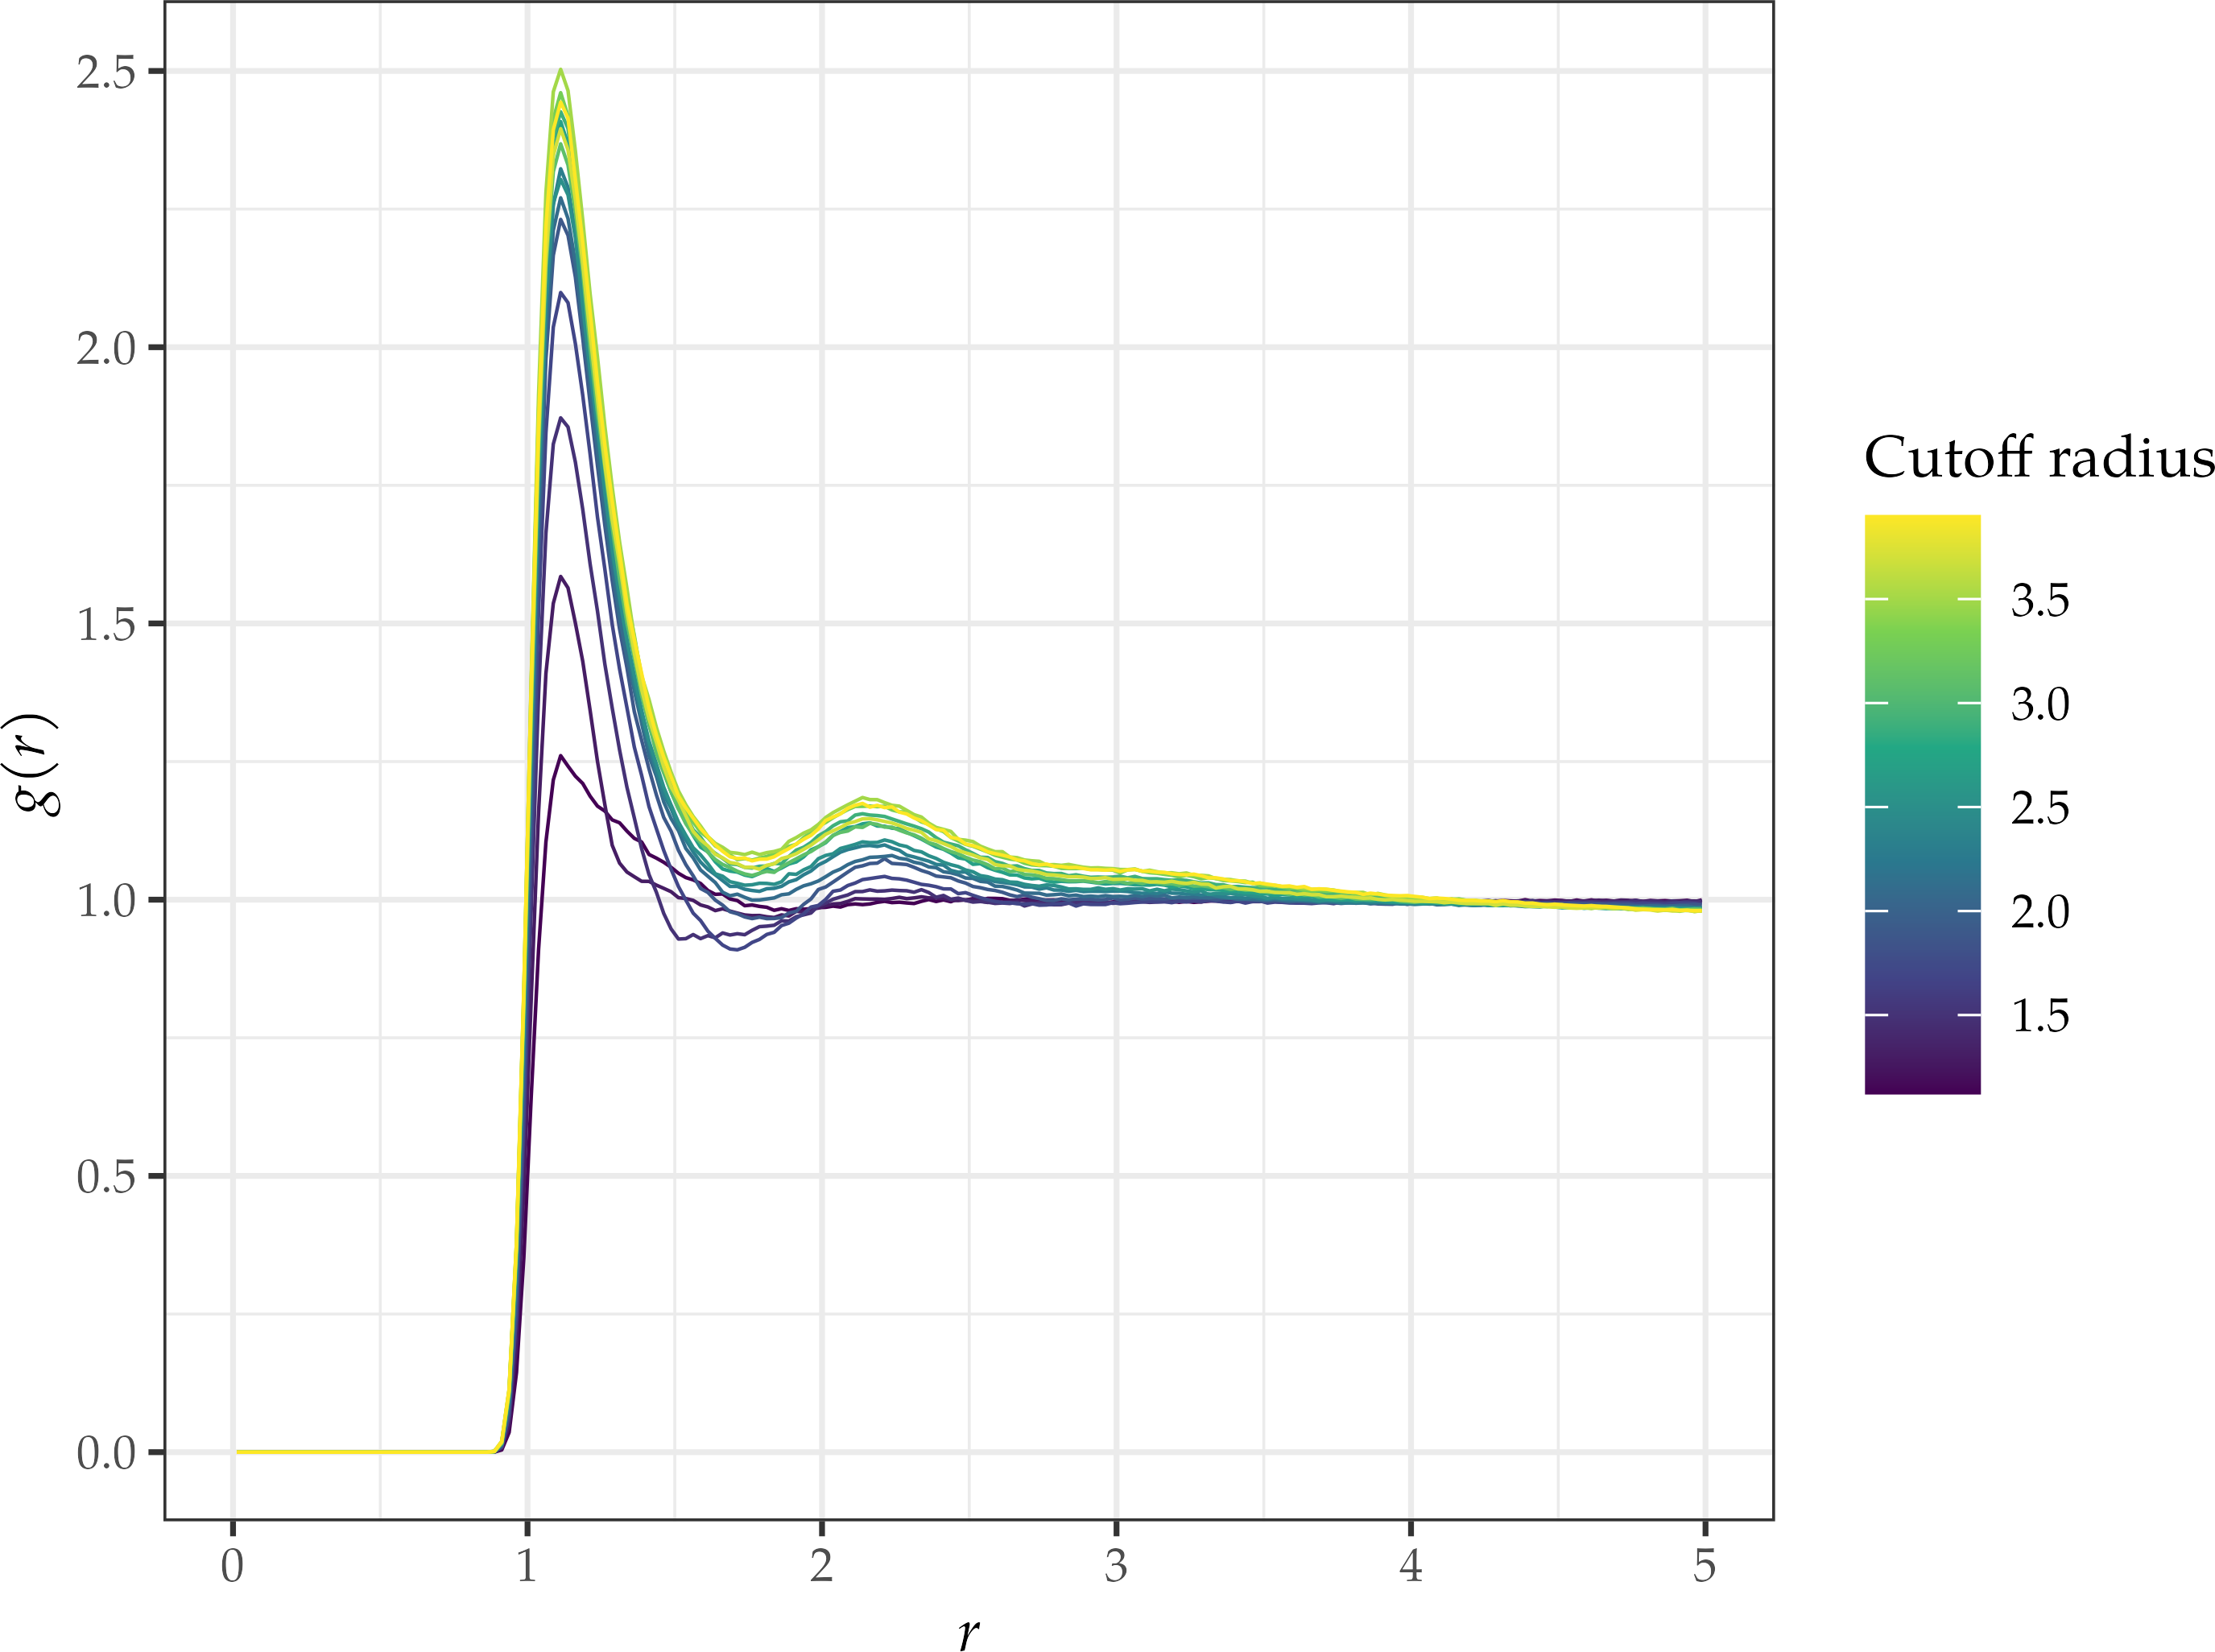
\includegraphics{img/102b}
  \caption{radial distribution function $g(r)$ at different cutoff radii for a
    Lennard-Jones system of \num{200} particles, box size $L = \num{10}$ and
    temperature $T = \num{1}$. Each line is the average over \num{10}
    realizations with \num{10000} \abbr{md} steps sampled every \num{10}, after
    an equilibration phase of \num{1000} \abbr{mc} sweeps.}
  \label{fig:102b}
\end{figure}

\begin{figure}
  \centering
  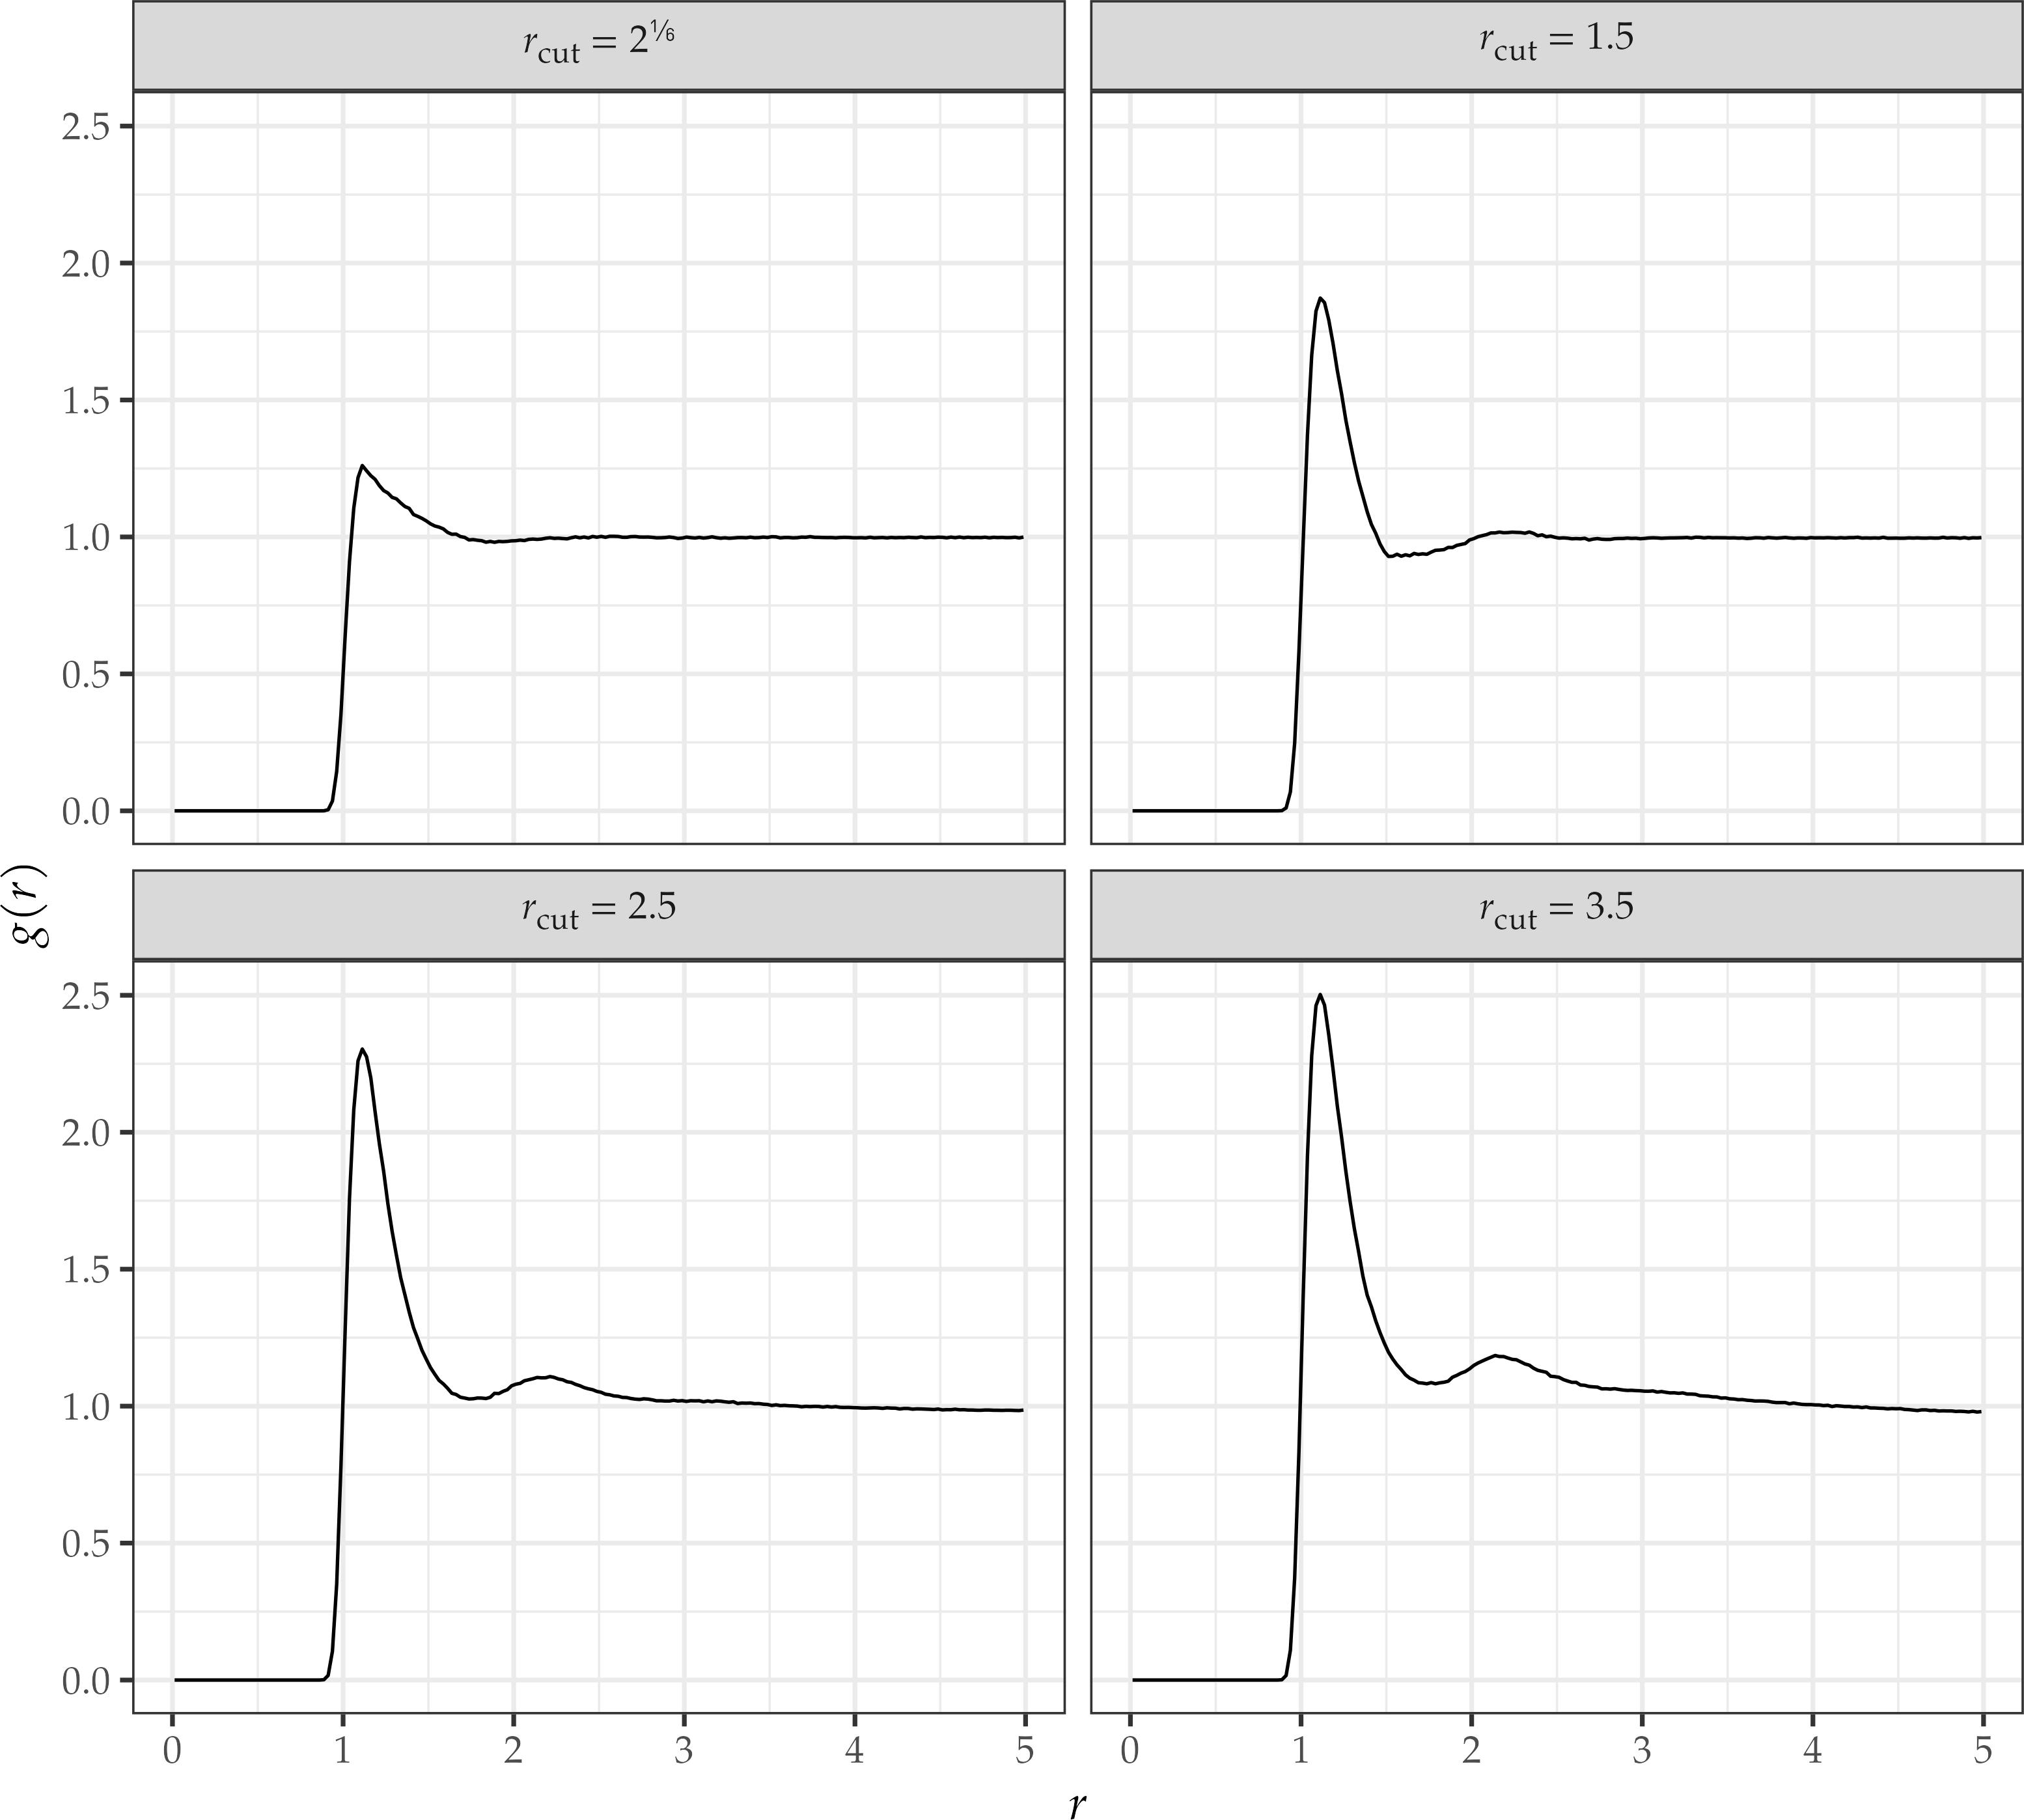
\includegraphics{img/102c}
  \caption{a selection of $g(r)$ profiles from \cref{fig:102b}.}
  \label{fig:102c}
\end{figure}
